\begin{figure*}[t!]
 
\begin{centering}

	\begin{subfigure}[b]{0.45\textwidth}
                \centering
                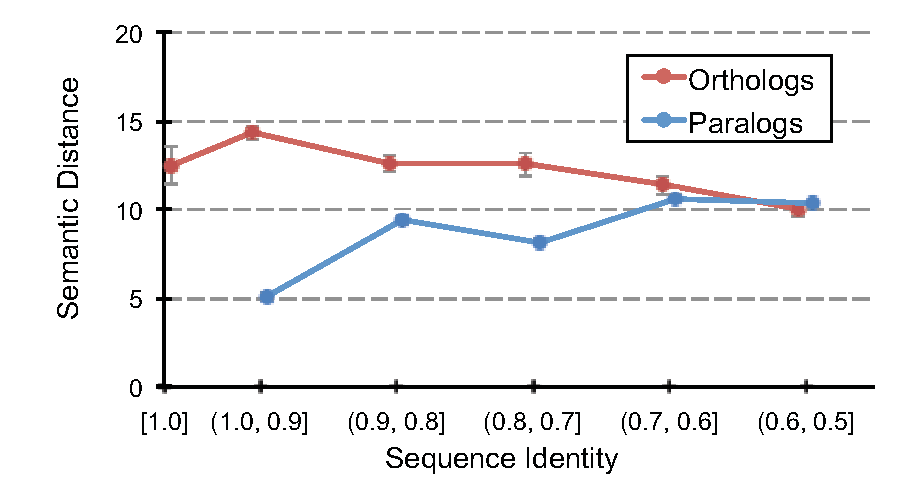
\includegraphics[width=\textwidth]{Figures/retesting/mfo_semantic_distance_unfiltered_2}
                \caption{$S_{2}$}
                \label{fig:unfilteredsd2}
        \end{subfigure}%
        \quad
	\begin{subfigure}[b]{0.45\textwidth}
                \centering
                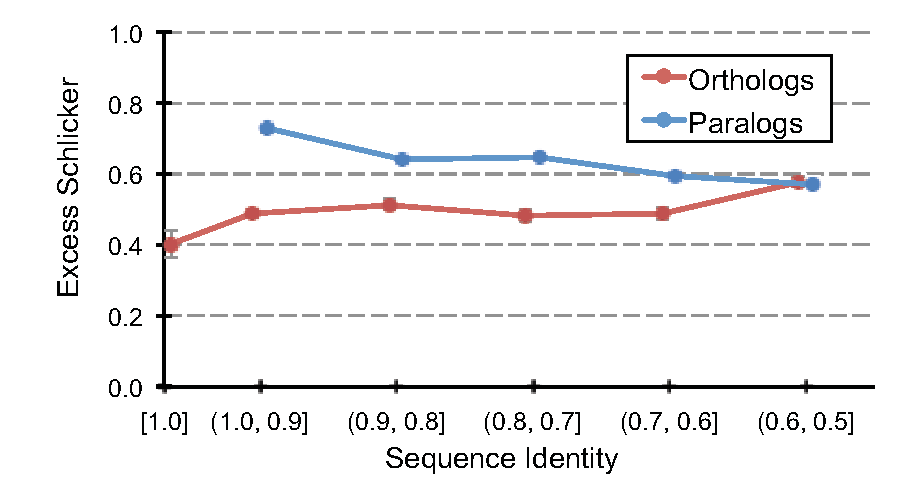
\includegraphics[width=\textwidth]{Figures/retesting/mfo_lin_unfiltered_2}
                \caption{Excess Schlicker}
                \label{fig:unfilteredlin2}
        \end{subfigure}
        
        	\begin{subfigure}[b]{0.45\textwidth}
                \centering
                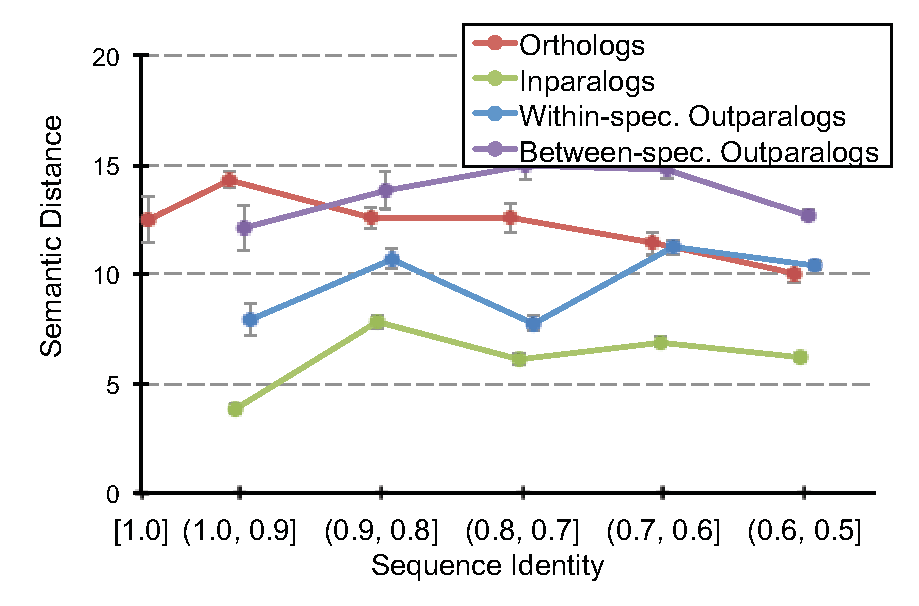
\includegraphics[width=\textwidth]{Figures/retesting/mfo_semantic_distance_unfiltered_4}
                \caption{$S_{2}$}
                \label{fig:unfilteredsd4}
        \end{subfigure}%
        \quad
	\begin{subfigure}[b]{0.45\textwidth}
                \centering
                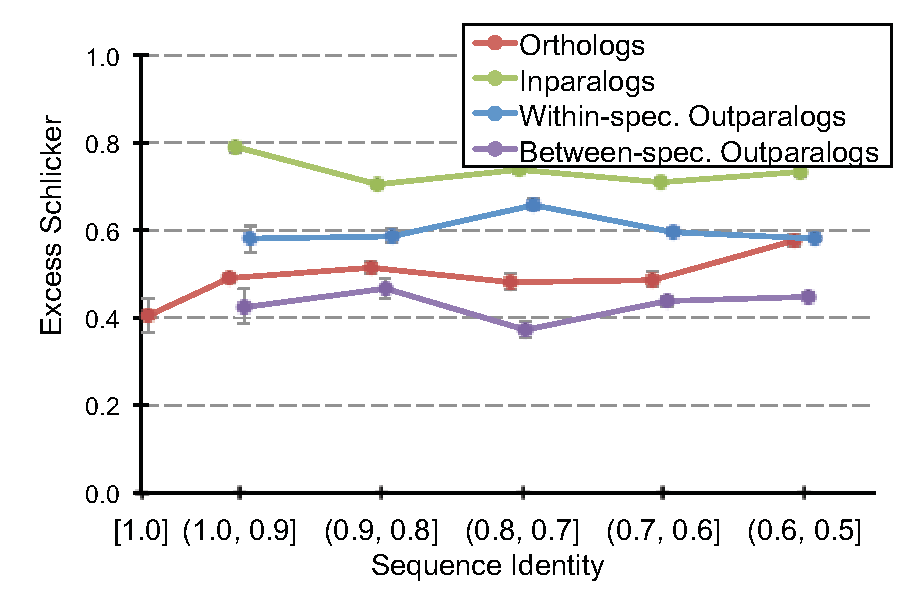
\includegraphics[width=\textwidth]{Figures/retesting/mfo_lin_unfiltered_4}
                \caption{Excess Schlicker}
                \label{fig:unfilteredlin4}
        \end{subfigure}

\end{centering}
\caption[Comparison of $S_{2}$ and ``Excess Schlicker"]{Comparison of $S_{2}$ and ``Excess Schlicker" for experimental molecular function annotations.  Results are not filtered for for common authorship, nor are they normalized based on the background similarity for each homology type and pair of organisms compared.}
\label{fig:unfiltered}
\end{figure*}

